\RequirePackage[l2tabu, orthodox]{nag}
\RequirePackage{silence}
\documentclass[french,english]{beamer}
\input{preamble/packages}
\input{preamble/math_basics}
\input{preamble/math_mine}
%Requires package xcolor.
\newcommand{\commentOC}[1]{\textcolor{blue}{\small$\big[$OC: #1$\big]$}}
%Requires package babel and option [french]. According to babel doc, need two braces around \selectlanguage to make the changes really local.
\newcommand{\commentOCf}[1]{\textcolor{blue}{{\small\selectlanguage{french}$\big[$OC : #1$\big]$}}}
\newcommand{\commentYM}[1]{\textcolor{red}{\small$\big[$YM: #1$\big]$}}
\newcommand{\commentYMf}[1]{\textcolor{red}{{\small\selectlanguage{french}$\big[$YM : #1$\big]$}}}

%TODO \crefname{axiom}{axiom}{axioms}%might be needed for workaround bug in cref when defining new theorems?
\crefname{examplex}{example}{examples}% I wonder why this is unnecessary in case of singular

%I find these settings useful in draft mode.
%Which line breaks are chosen: accept worse lines, therefore reducing risk of overfull lines. Default = 200.
	\tolerance=2000
%Accept overfull hbox up to...
	\hfuzz=2cm
%Reduces verbosity about the bad line breaks.
	\hbadness 5000
%Reduces verbosity about the underful vboxes.
	\vbadness=1300

\bibliographystyle{abbrvnat}

%TODO test the brackets.
%\newcommand{\llbracket}{\lbrack\!\lbrack}
%\newcommand{\rrbracket}{\rbrack\!\rbrack}

%2212 Minus Sign
\newunicodechar{−}{\ifmmode{-}\else\textminus\fi}
%These symbols can only be used in math mode, for I found no text equivalent.
%03B3 Greek Small Letter Gamma
\newunicodechar{γ}{\gamma}
%03B4 Greek Small Letter Delta
\newunicodechar{δ}{\delta}
%2115 Double-Struck Capital N
\newunicodechar{ℕ}{\mathbb{N}}
%211D Double-Struck Capital R
\newunicodechar{ℝ}{\mathbb{R}}
%21CF Rightwards Double Arrow with Stroke
\newunicodechar{⇏}{\nRightarrow}
%21D2 Rightwards Double Arrow
\newunicodechar{⇒}{\Rightarrow}
%21D4 Left Right Double Arrow
\newunicodechar{⇔}{\Leftrightarrow}
%2227 Logical And
\newunicodechar{∧}{\land}
%2228 Logical Or
\newunicodechar{∨}{\lor}
%2229 Intersection
\newunicodechar{∩}{\cap}
%222A Union
\newunicodechar{∪}{\cup}
%2260 Not Equal To
\newunicodechar{≠}{\neq}
%2264 Less-Than or Equal To
\newunicodechar{≤}{\leq}
%2265 Greater-Than or Equal To
\newunicodechar{≥}{\geq}
%227B Succeeds
\newunicodechar{≻}{\succ}
%2281 Does Not Succeed
\newunicodechar{⊁}{\nsucc}
%22EB Does Not Contain As Normal Subgroup
\newunicodechar{⋫}{\ntriangleright}
%25A1 White Square
\newunicodechar{□}{\Box}
%25B7 White Right-Pointing Triangle
%TODO test \rhd; \ntrianglerighteq from amssymb?
\newunicodechar{▷}{\triangleright}
%27E6 Mathematical Left White Square Bracket – there’s also \llbracket from stmaryrd
\newunicodechar{⟦}{\text{\textlbrackdbl}}
%27E7 Mathematical Right White Square Bracket – there’s also \rrbracket from stmaryrd
\newunicodechar{⟧}{\text{\textrbrackdbl}}
%27FC Long Rightwards Arrow from Bar
\newunicodechar{⟼}{\longmapsto}
%2AB0 Succeeds Above Single-Line Equals Sign
\newunicodechar{⪰}{\succeq}
%301A Left White Square Bracket
\newunicodechar{〚}{\textlbrackdbl}
%301B Right White Square Bracket
\newunicodechar{〛}{\textrbrackdbl}
%→ is defined by default as \textrightarrow, which is invalid in math mode. Same thing for the three other commands. I redefine those four using \DeclareUnicodeCharacter instead of \newunicodechar because the latter warns about the previous definition.
%→ Rightwards Arrow
\DeclareUnicodeCharacter{2192}{\ifmmode\rightarrow\else\textrightarrow\fi}
%¬ Not Sign
\DeclareUnicodeCharacter{00AC}{\ifmmode\lnot\else\textlnot\fi}
%… Horizontal Ellipsis
\DeclareUnicodeCharacter{2026}{\ifmmode\dots\else\textellipsis\fi}
%× Multiplication Sign
\DeclareUnicodeCharacter{00D7}{\ifmmode\times\else\texttimes\fi}


\input{preamble/draw}
\DeclareAcronym{AMCD}{short=amcd, long={Aide Multicritère à la Décision}}
\DeclareAcronym{AR}{short=ar, long={Argumentative Recommender}}
\DeclareAcronym{DA}{short=da, long={Decision Analysis}}
\DeclareAcronym{DM}{short=dm, long={Decision Maker}}
\DeclareAcronym{DP}{short=dp, long={Deliberated Preference}}
\DeclareAcronym{MAVT}{short=mavt, long={Multiple Attribute Value Theory}}
\DeclareAcronym{MCDA}{short=mcda, long={Multicriteria Decision Aid}}
\DeclareAcronym{MIP}{short=mip, long={Mixed Integer Program}}



\setbeamertemplate{headline}[singleline]

\title{Learning argumentative recommenders}
\subject{Argumentation}
\keywords{Machine Learning, MCDM, MCDA, Utility Theory}
\author{Olivier Cailloux}
\institute[LAMSADE]{LAMSADE, Université Paris-Dauphine}
\date{\formatdate{22}{11}{2018}}

\begin{document}
\begin{frame}[plain]
	\tikz[remember picture,overlay]{
		\path (current page.south west) node[anchor=south west, inner sep=0] {
			\includegraphics[height=1cm]{LAMSADE95.jpg}
		};
		\path (current page.south) ++ (0, 1mm) node[anchor=south, inner sep=0] {
			\includegraphics[height=9mm]{Dauphine.jpg}
		};
		\path (current page.south east) node[anchor=south east, inner sep=0] {
			\includegraphics[height=1cm]{PSL.png}
		};
		\path (current page.south) ++ (0, 4em) node[anchor=south, inner sep=0] {
			\scriptsize\color{blue}\url{https://github.com/oliviercailloux/CLut}
		};
%thanks to https://stackoverflow.com/questions/2423777/is-it-possible-to-create-a-remote-repo-on-github-from-the-cli-without-opening-br/13366414#13366414
%REPO=…
%curl -u 'oliviercailloux' https://api.github.com/user/repos -d "{\"name\":\"${REPO}\"}"
%git remote add origin git@github.com:oliviercailloux/${REPO}.git
%git push --set-upstream origin master
	}
	\titlepage
\end{frame}
\addtocounter{framenumber}{-1}

\begin{frame}
	\frametitle{A new goal}
	\begin{itemize}
		\item Recommender systems: what’s appropriate for $i$?
		\item Appropriate, classically: among top-preferred
		\item Appropriate, here: among the \acl{DP} of $i$
	\end{itemize}
	\begin{block}{\ac{DP}}
		Choice behavior when $i$ has taken all arguments into account to form a deliberated opinion
	\end{block}
\end{frame}

\begin{frame}
	\frametitle{Outline}
	\tableofcontents[hideallsubsections, sectionstyle=shaded/show]
\end{frame}

\AtBeginSection{
	\begin{frame}
		\frametitle{Outline}
		\tableofcontents[currentsection, hideallsubsections]
	\end{frame}
}

\section{Motivation}
\begin{frame}
	\frametitle{Two sorts of preference}
	\begin{block}{Intuitive preference}
		\begin{itemize}
			\item Preference as an “immediate sensation” \citep{von_neumann_theory_1944}
			\item $i$ knows what’s best by introspection
			\item Recommend a movie: $i$ knows how good it feels
			\item “There is, of course, an important sense in which preferences, being entirely subjective, cannot be in error” \citep{savage_foundations_1972}
		\end{itemize}
	\end{block}
	\begin{block}{Deliberated preference}
		\begin{itemize}
			\item … “but in a different, more subtle sense they can be.”
			\item On reflection, I change my mind
			\item Relates to “slow thinking” \citep{kahneman_thinking_2013}
		\end{itemize}
	\end{block}
\end{frame}

\begin{frame}
	\frametitle{Relevance}
	Appropriate when desired to help $i$ deliberate
	\begin{itemize}
		\item Can’t try out the items (non repeatable choice)
		\item Finding best requires careful consideration of all arguments
	\end{itemize}
	Examples:
	\begin{itemize}
		\item Choice of place of study
		\item Which smartphone / house to buy? 
		\item How to distribute a prize or revenue? (Fairness?)
		\item To which cause should I donate money?
	\end{itemize}
	\begin{exampleblock}{Example: A decision procedure for credit requests in a bank}
		\begin{itemize}
			\item Fairness (unconscious discrimination?)
			\item Go beyond reflecting some expert’s intuition
		\end{itemize}
	\end{exampleblock}
\end{frame}

\section{\acl{DP}}
\begin{frame}
	\frametitle{Context}
	\begin{description}
		\item[$\allitems$] The possible items 
		\item[$\allargs$] All arguments 
		\item[$\ar \in \allargs$] An argument (a text in English)
	\end{description}
	\begin{exampleblock}{Example argument}
		Item $\itm$ is better than item $\itm'$ because $\itm$ has a good performance on criteria ‘price’ and ‘speed’ while item $\itm'$ has a good performance only on criterion ‘aspect’, which you do not consider important
	\end{exampleblock}
\end{frame}

\begin{frame}
	\frametitle{Attitude towards arguments and \acl{DP}}
	\begin{itemize}
		\item Given $\ar$ in favor of $\itm$; $\ar'$ in favor of $\itm'$
		\item Does $i$ prefer $\itm$ or $\itm'$?
		\item $\ibeats$ binary relation over $\allitems × \allargs$: $(\itm, \ar) \ibeats (\itm', \ar')$ iff $\usr$ strictly prefers $\itm$ to $\itm'$, given $\ar$ and $\ar'$
		\item $\uitems \subseteq \allitems$, the items in the \ac{DP} of $i$: having no items strictly preferred to them, \emph{all arguments considered}
	\end{itemize}
	\begin{block}{\acl{DP}}
		$\itm \in \uitems$ iff
		\begin{equation}
			\forall (\itm', \ar') \in \allitems × \allargs, \exists \ar \in \allargs \suchthat (\itm', \ar') \nibeats (\itm, \ar)
		\end{equation}
	\end{block}
\end{frame}

\section{\aclp{AR}}
\begin{frame}
	\frametitle{\acl{AR}}
	\begin{block}{Goal of an \ac{AR}}
		\begin{itemize}
			\item Exhibit some items $\itm \in \uitems$ and some $\itm' \notin \uitems$
			\item Argue for those claims
		\end{itemize}
	\end{block}
	Given $i$, \ac{AR} $\eta$ produces:
	\begin{description}[$\mdef: \mitems × \allitems → \allargs$]
		\item[$\mitems \subseteq \allitems$] items that $\eta$ claims are in $\uitems$
		\item[$\mdef: \mitems × \allitems → \allargs$] to defend items in $\mitems$
		\item[$R_\eta \subseteq \allitems × \allitems$] pairs $(\itm, \itm')$ such that $\eta$ claims that $\usr$ deliberately prefers $\itm$ to $\itm'$
		\item[$\matt: R_\eta → \allargs$] to support the claims represented by $R_\eta$
	\end{description}
	Permits to compare ARs!
\end{frame}

\section{Convergence with \acl{DA}}
\begin{frame}
	\frametitle{Relationship with \acl{DA}}
	\begin{itemize}
		\item \ac{DA} has a similar goal: help user deliberate
		\item DA use preference models based on sound principles
		\item Models not perfectly accurate to describe everyday behavior
		\item But might better describe thoughtful behavior
		\item Prospect theory \citep{wakker_prospect_2010} VS Utility theory
	\end{itemize}
\end{frame}

\begin{frame}
	\frametitle{Build \aclp{AR} with \acl{DA} models}
	\begin{itemize}
		\item Search models of \ac{DP} within a class of models proposed in \ac{DA}
		\item Use and extend work producing arguments given \ac{DA} models
	\end{itemize}
\end{frame}

\begin{frame}
	\frametitle{EU maximizer facing Allais’s problem}
	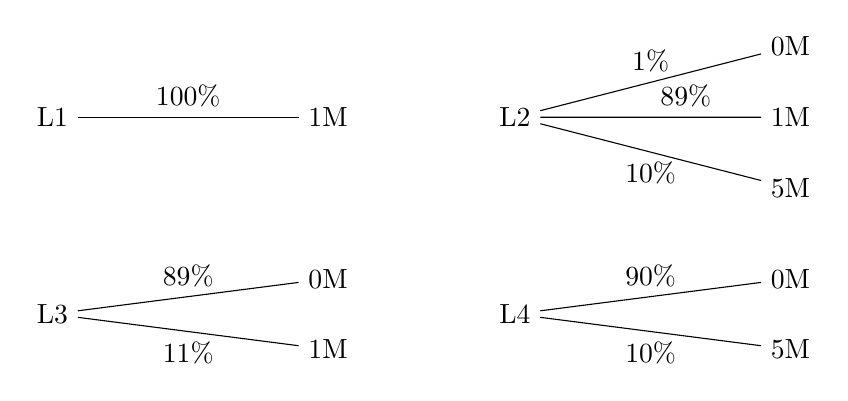
\begin{tikzpicture}[grow'=right, sibling distance=9mm, level distance=35mm]
		\path node (l1) {L1} child {
			node {1M} edge from parent node[above] {100\%}
		};
		\path (l1-1.east) ++ (2cm, 0) node (l2) {L2} child {
			node {0M} edge from parent node[above] {1\%}
		} child {
			node {1M} edge from parent node[above right] {89\%}
		} child {
			node {5M} edge from parent node[below] {10\%}
		};
		\path (l1) ++(0, -25mm) node (l3) {L3} child {
			node {0M} edge from parent node[above] {89\%}
		} child {
			node {1M} edge from parent node[below] {11\%}
		};
		\path (l3 -| l2) node (l4) {L4} child {
			node {0M} edge from parent node[above] {90\%}
		} child {
			node {5M} edge from parent node[below] {10\%}
		};
	\end{tikzpicture}
	\begin{itemize}
		\item $i$ could be intuitively attracted by L1 $\succ$ L2 and L3 $\succ$ L4
		\item Expected Utility principles could help
		\item … if $i$ is a utility maximizer
		\item Prescription useful to Savage himself
	\end{itemize}
\end{frame}

\begin{frame}
	\frametitle{Conclusion}
	\begin{itemize}
		\item To help $i$ decide
		\item Build \aclp{AR}
		\item Still a prediction problem:
		\item predict her \acl{DP}
		\item To be done using \acl{DA} principles or otherwise!
	\end{itemize}
\end{frame}

\begin{frame}[plain]
	\addtocounter{framenumber}{-1}
	\begin{center}
		\huge
		\textit{Thank you for your attention!}
	\end{center}
\end{frame}

\appendix
\AtBeginSection{
}

\clearpage\pdfbookmark[2]{\refname}{\refname}
\begin{frame}[allowframebreaks]
	\frametitle{\refname}
 	\bibliography{manual}
\end{frame}

\section{Various}
\begin{frame}
	\frametitle{Thierry’s problem}
	Thierry wants to choose a car!
	\begin{block}{Example recommendation}
		\begin{itemize}
			\item Like speed? Pick $A$
			\item Like comfort? Pick $B$
			\item Don’t take $C$: bad tradeoff
		\end{itemize}
	\end{block}
	\begin{block}{Good advice?}
		\begin{itemize}
			\item Wrt \ac{DP}
			\item Empirical question
			\item Uses psychology of Thierry or of humans (Consumers Report strategy)
		\end{itemize}
	\end{block}
\end{frame}

\clearpage\pdfbookmark{License}{License}
\begin{frame}[plain]
	\frametitle{License}
	This presentation, and the associated \LaTeX{} code, are published under the \href{http://opensource.org/licenses/MIT}{MIT license}. Feel free to reuse (parts of) the presentation, under condition that you cite the author.
	
	Credits are to be given to \href{http://www.lamsade.dauphine.fr/~ocailloux/}{Olivier Cailloux}, Université Paris-Dauphine.
\end{frame}
\addtocounter{framenumber}{-1}
\end{document}

\begin{frame}
	\frametitle{}
	\begin{itemize}
		\item 
	\end{itemize}
\end{frame}

